%%%%%%%%%%%%%%%%%%%%%%%%%%%%%%%%%%%%%%%%%
%
% Author: Fabrizio Zeni
%
%%%%%%%%%%%%%%%%%%%%%%%%%%%%%%%%%%%%%%%%%

%----------------------------------------------------------------------------------------
%	PACKAGES AND OTHER DOCUMENT CONFIGURATIONS
%----------------------------------------------------------------------------------------

\documentclass{article}

\usepackage{fancyhdr} % Required for custom headers
\usepackage{lastpage} % Required to determine the last page for the footer
\usepackage{extramarks} % Required for headers and footers
\usepackage[usenames,dvipsnames]{color} % Required for custom colors
\usepackage{graphicx} % Required to insert images
\usepackage{listings} % Required for insertion of code
\usepackage{courier} % Required for the courier font
\usepackage{lipsum} % Used for inserting dummy 'Lorem ipsum' text into the template
\usepackage{caption}


\definecolor{mygreen}{rgb}{0,0.6,0}
\definecolor{mygray}{rgb}{0.5,0.5,0.5}
\definecolor{mymauve}{rgb}{0.58,0,0.82}


% Margins
\topmargin=-0.45in
\evensidemargin=0in
\oddsidemargin=0in
\textwidth=6.5in
\textheight=9.0in
\headsep=0.25in

\linespread{1.1} % Line spacing

% Set up the header and footer
\pagestyle{fancy}
\lhead{\hmwkAuthorName} % Top left header
\chead{\hmwkClass\ : \hmwkTitle} % Top center head
%\rhead{\firstxmark} % Top right header
\lfoot{\lastxmark} % Bottom left footer
\cfoot{} % Bottom center footer
\rfoot{Page\ \thepage\ of\ \protect\pageref{LastPage}} % Bottom right footer
\renewcommand\headrulewidth{0.4pt} % Size of the header rule
\renewcommand\footrulewidth{0.4pt} % Size of the footer rule

\setlength\parindent{0pt} % Removes all indentation from paragraphs

%----------------------------------------------------------------------------------------
%	CODE INCLUSION CONFIGURATION
%----------------------------------------------------------------------------------------

\definecolor{MyDarkGreen}{rgb}{0.0,0.4,0.0} % This is the color used for comments
\lstloadlanguages{PHP,Java,Sql,HTML} % Load Perl syntax for listings, for a list of other languages supported see: ftp://ftp.tex.ac.uk/tex-archive/macros/latex/contrib/listings/listings.pdf

\lstset{ %
  backgroundcolor=\color{SpringGreen},   % choose the background color; you must add \usepackage{color} or \usepackage{xcolor}
  basicstyle=\footnotesize,        % the size of the fonts that are used for the code
  breakatwhitespace=false,         % sets if automatic breaks should only happen at whitespace
  breaklines=true,                 % sets automatic line breaking
  captionpos=b,                    % sets the caption-position to bottom
  commentstyle=\color{mygreen},    % comment style
  deletekeywords={...},            % if you want to delete keywords from the given language
  escapeinside={\%*}{*)},          % if you want to add LaTeX within your code
  extendedchars=true,              % lets you use non-ASCII characters; for 8-bits encodings only, does not work with UTF-8
  frame=single,                    % adds a frame around the code
  keywordstyle=\color{blue},       % keyword style
  language=PHP,                 % the language of the code
  morekeywords={*,...},            % if you want to add more keywords to the set
  numbers=left,                    % where to put the line-numbers; possible values are (none, left, right)
  numbersep=5pt,                   % how far the line-numbers are from the code
  stepnumber=3,    
  firstnumber=1,
  numberfirstline=false
  %numberstyle=\tiny\color{gray}, % the style that is used for the line-numbers
  rulecolor=\color{black},         % if not set, the frame-color may be changed on line-breaks within not-black text (e.g. comments (green here))
  showspaces=false,                % show spaces everywhere adding particular underscores; it overrides 'showstringspaces'
  showstringspaces=false,          % underline spaces within strings only
  showtabs=false,                  % show tabs within strings adding particular underscores
  %stepnumber=2,                    % the step between two line-numbers. If it's 1, each line will be numbered
  stringstyle=\color{mymauve},     % string literal style
  tabsize=2,                       % sets default tabsize to 2 spaces
  title=\lstname                   % show the filename of files included with \lstinputlisting; also try caption instead of title
}


% Creates a new command to include a perl script, the first parameter is the filename of the script (without .pl), the second parameter is the caption
\newcommand{\phpscript}[1]{
\begin{itemize}
%\item[]\lstinputlisting[caption=#2,label=#2,firstline=#3,lastline=#4]{#1.php}
\item[]\lstinputlisting{/var/www/sm/#1.php}
\end{itemize}
}

%----------------------------------------------------------------------------------------
%	DOCUMENT STRUCTURE COMMANDS
%	Skip this unless you know what you're doing
%----------------------------------------------------------------------------------------

% Header and footer for when a page split occurs within a problem environment
\newcommand{\enterProblemHeader}[1]{
\nobreak\extramarks{#1}{#1 continued on next page\ldots}\nobreak
\nobreak\extramarks{#1 (continued)}{#1 continued on next page\ldots}\nobreak
}

% Header and footer for when a page split occurs between problem environments
\newcommand{\exitProblemHeader}[1]{
\nobreak\extramarks{#1 (continued)}{#1 continued on next page\ldots}\nobreak
\nobreak\extramarks{#1}{}\nobreak
}

\setcounter{secnumdepth}{0} % Removes default section numbers
\newcounter{homeworkProblemCounter} % Creates a counter to keep track of the number of problems

\newcommand{\homeworkProblemName}{}
\newenvironment{homeworkProblem}[1]{ % Makes a new environment called homeworkProblem which takes 1 argument (custom name) but the default is "Problem #"
%[Problem \arabic{homeworkProblemCounter}]
%\stepcounter{homeworkProblemCounter} % Increase counter for number of problems
\renewcommand{\homeworkProblemName}{#1} % Assign \homeworkProblemName the name of the problem
\begin{center}
\section{#1} % Make a section in the document with the custom problem count
\end{center}
\enterProblemHeader{#1} % Header and footer within the environment
%\exitProblemHeader{\homeworkProblemName}
}{
\exitProblemHeader{\homeworkProblemName} % Header and footer after the environment
}

\newcommand{\problemAnswer}[1]{ % Defines the problem answer command with the content as the only argument
\noindent\framebox[\columnwidth][c]{\begin{minipage}{0.98\columnwidth}#1\end{minipage}} % Makes the box around the problem answer and puts the content inside
}

\newcommand{\homeworkSectionName}{}
\newenvironment{homeworkSection}[1]{ % New environment for sections within homework problems, takes 1 argument - the name of the section
\renewcommand{\homeworkSectionName}{#1} % Assign \homeworkSectionName to the name of the section from the environment argument
\subsection{\homeworkSectionName} % Make a subsection with the custom name of the subsection
\enterProblemHeader{"asdasd"\ [\homeworkSectionName]}
%\enterProblemHeader{\homeworkProblemName\ [\homeworkSectionName]} % Header and footer within the environment
}
%{
%\enterProblemHeader{\homeworkProblemName} % Header and footer after the environment
%}

%----------------------------------------------------------------------------------------
%	NAME AND CLASS SECTION
%----------------------------------------------------------------------------------------

\newcommand{\hmwkTitle}{Assignment\ \#8} % Assignment title
\newcommand{\hmwkSubTitle}{Security Test Cases} %Subtitle
\newcommand{\hmwkDueDate}{Friday,\ April\ 19,\ 2013} % Due date
\newcommand{\hmwkClass}{Security\ Testing} % Course/class
%\newcommand{\hmwkClassTime}{13:30am} % Class/lecture time
%\newcommand{\hmwkClassInstructor}{Jones} % Teacher/lecturer
\newcommand{\hmwkAuthorName}{Fabrizio\ Zeni} % Your name
\newcommand{\hmwkAuthorSId}{Student Id: 153465} % Student Id

%----------------------------------------------------------------------------------------
%	TITLE PAGE
%----------------------------------------------------------------------------------------

\title{
\vspace{2in}
\textmd{\textbf{\hmwkClass:\ \hmwkTitle}}\\
\textmd{\normalsize{\textbf{\hmwkSubTitle}}}\\
%\normalsize\vspace{0.1in}\small{Due\ on\ \hmwkDueDate}\\
%\vspace{0.1in}\large{\textit{\hmwkClassInstructor\ \hmwkClassTime}}
\vspace{3in}
}

\author{\textbf{\hmwkAuthorName} \\ \small{\hmwkAuthorSId}}
\date{} % Insert date here if you want it to appear below your name

%----------------------------------------------------------------------------------------

\begin{document}

\maketitle

%----------------------------------------------------------------------------------------
%	TABLE OF CONTENTS
%----------------------------------------------------------------------------------------

%\setcounter{tocdepth}{1} % Uncomment this line if you don't want subsections listed in the ToC

\newpage
\tableofcontents
\newpage

%----------------------------------------------------------------------------------------
%	VULNERABILITY 11
%----------------------------------------------------------------------------------------

\begin{homeworkProblem}{Vulnerability 11}
\label{sec:V11}
\subsection{Brief Analysis}
\begin{center}
	File: AddAssignment.php
\\Similar Vulnerabilities\footnote{their test cases are based on the ones of this vulnerability}: \\16,18,19,63,70,71,87,88,89,90,93,126,138,141,165,180,181,186,194,200,201,230,238,269,272,316
	\begin{table}[h]
		\begin{center}
    		\begin{tabular}{ | c | c |}
    			\hline
    			\textbf{VARIABLE} & \textbf{RESULT} \\ \hline
  				page & true \\ \hline
  				page2 & true \\ \hline
  				selectclass & true \\ \hline
    		\end{tabular}
    	\end{center}
   \end{table}
\end{center}
\subsection{JWebUnit test cases}
\subsubsection{prepare and cleanup}
\begin{lstlisting}[language=Java,caption=prepare function]
	public void prepare(){
        tester = new WebTester();
        tester.setBaseUrl("http://localhost/sm/");
        tester.beginAt("index.php");
        Functions.login(tester,"teacher");
        Functions.click(tester,"Music",0);
        tester.assertMatch("Class Settings");
        Functions.click(tester,"Assignments",0);
        tester.assertMatch("Manage Assignments");
	}
\end{lstlisting}
\begin{lstlisting}[language=Java,caption=cleanup function]
	public void cleanup(){
		Functions.click(tester,"Log Out",0);
		tester = null;
	}
\end{lstlisting}
In these two functions there is nothing special, just navigation and call to the login/logout utilities.
\begin{center}
	\textit{\small Continues on the next page ...}
\end{center}
\clearpage
\subsubsection{page}
\begin{lstlisting}[language=Java,caption=jwebunit test code for \textit{page}]
	public void page(){
		Vulnerabilities.page(tester,"assignments","Add");
        tester.assertMatch("Add New Assignment");
        tester.assertLinkNotPresentWithText("malicious");
	}
\end{lstlisting}
\begin{lstlisting}[language=Java,caption=function for the \textit{page} vulnerability]
	public static void page(WebTester tester,String formName,String buttonName){
        IElement page = tester.getElementByXPath("//form[@name='" + formName + "']//input[@name='page']");
        String oldValue = page.getAttribute("value");
        page.setAttribute("value",oldValue +"'><a href='http://www.unitn.it'>malicious</a><br'");
        if(buttonName!=null)
        	Functions.click(tester,buttonName,1);
	}
\end{lstlisting}
This code does the test for \textit{page}. In order to catch the correct hidden field it was necessary to filter the form first, because there were two hidden fields with the same name and the first is not the one triggered by the buttons.
So the function retrieves the page2 input element and stores it into the \emph{oldValue} variable, which at line 6 is concatenated to the malicious link and inserted into the page value.
\subsubsection{page2}
\begin{lstlisting}[language=Java,caption=jwebunit test code for \textit{page2}]
	public void page2(){
		Vulnerabilities.page2(tester,"assignments","Add");
        tester.assertMatch("Add New Assignment");
        tester.assertLinkNotPresentWithText("malicious");
	}
\end{lstlisting}
\begin{lstlisting}[language=Java,caption=function for the \textit{page2} vulnerability]
	public static void page2(WebTester tester,String formName,String buttonName){
		IElement page2 = tester.getElementByXPath("//form[@name='" + formName + "']//input[@name='page2']");
		IElement button = tester.getElementByXPath("//input [@value='" + buttonName + "']");
		String onClick = button.getAttribute("onClick");
		String[] fixedValues = Functions.page2Fix(formName, onClick);
		fixedValues[0] = fixedValues[0].replace("'","");
		page2.setAttribute("value",fixedValues[0] + "'><a href='http://www.unitn.it'>malicious</a><br'");
		button.setAttribute("onClick",fixedValues[1]);
		Functions.click(tester,buttonName,1);
	}
\end{lstlisting}
The page2 vulnerability was more subtle to automatically trigger. That was due to the fact that the form buttons have a \textit{javascript} code in the attribute \textbf{onClick}, which write on the page2 value. So that in order to prevent the button from modify the injected value, at line 3 the button element is retrieved, then we get the value of the onClick attribute, which is processed by the \emph{page2Fix function} -  which purge the attribute from any command that modifies the page2 value and returns the value for page2 and the other instructions that need to be put back into the attribute.
\subsubsection{selectclass}
\begin{lstlisting}[language=Java,caption=jwebunit test code for \textit{selectclass}]
	public void selectclass(){
		Vulnerabilities.selectclass(tester,"assignments","Add");
        tester.assertMatch("Add New Assignment");
        tester.assertLinkNotPresentWithText("malicious");
	}
\end{lstlisting}
\begin{lstlisting}[language=Java,caption=function for the \textit{selectclass} vulnerability]
	public static void selectclass(WebTester tester,String formName,String buttonName){
        IElement selectclass = tester.getElementByXPath("//form[@name='" + formName + "']//input[@name='selectclass']");
        String oldValue = selectclass.getAttribute("value");
        selectclass.setAttribute("value",oldValue+"'><a href='http://www.unitn.it'>malicious</a><br'");
        Functions.click(tester,buttonName,1);
	}
\end{lstlisting}
The selectclass vulnerability was almost straightforward and differs from the \textit{page} function just in the attribute name in the XPath expression. 
\end{homeworkProblem}
\clearpage

%----------------------------------------------------------------------------------------
%	VULNERABILITY 13
%----------------------------------------------------------------------------------------

\begin{homeworkProblem}{Vulnerability 13}
\label{sec:V13}
\subsection{Brief Analysis}
\begin{center}
	File: AddAttendance.php
\\Similar Vulnerabilities\footnote{their test cases are based on the ones of this vulnerability}: 194
	\begin{table}[h]
		\begin{center}
    		\begin{tabular}{ | c | c | }
    			\hline
    			\textbf{VARIABLE} & \textbf{RESULT} \\ \hline
  				page & true \\ \hline
  				page2 & true \\ \hline
  				student & true \\ \hline
  				semester & true \\ \hline
    		\end{tabular}
    	\end{center}
   \end{table}
\end{center}
\subsection{JWebUnit test cases}
\subsubsection{prepare and cleanup}
\begin{lstlisting}[language=Java,caption=prepare function]
	public void prepare(){
        tester = new WebTester();
        tester.setBaseUrl("http://localhost/sm/");
        tester.beginAt("index.php");
        Functions.login(tester,"admin");
		Functions.click(tester,"Attendance",0);
		tester.assertMatch("Tardy");
	}
\end{lstlisting}
\begin{lstlisting}[language=Java,caption=cleanup function]
	public void cleanup(){
		Functions.click(tester,"Log Out",0);
		tester = null;
	}
\end{lstlisting}
\subsubsection{page and page2}
The code is adapted from the one of \textit{Vulnerability 11} at page ~\pageref{sec:V11}
\subsubsection{student}
\begin{lstlisting}[language=Java,caption=jwebunit test code for \textit{student}]
	public void student(){
		Vulnerabilities.selectInputVulnerability(tester,"registration","Add","student");
        tester.assertMatch("Add New Attendance Record");
        tester.assertLinkNotPresentWithText("malicious");
	}
\end{lstlisting}
\begin{lstlisting}[language=Java,caption=function for vulnerabilities over select input elements]
	public static void selectInputVulnerability(WebTester tester,String formName,String buttonName,String vulnerability){
		IElement selectInput = tester.getElementByXPath("//form[@name='" + formName +
				"']//select[@name='" + vulnerability + "']//option[@selected]");
        String oldValue = selectInput.getAttribute("value");
        selectInput.setAttribute("value",oldValue+"'><a href='http://www.unitn.it'>malicious</a><br /'");
        Functions.click(tester,buttonName,1);
	}
\end{lstlisting}
In this case the input element was a \textbf{select}, so the XPATH expression was modified with \emph{//option[@selected]} to catch the selected option. The remaining part of the code is almost equivalent to the \textit{page} one.
\subsubsection{semester}
\begin{lstlisting}[language=Java,caption=jwebunit test code for \textit{semester}]
	public void semester(){
		Vulnerabilities.selectInputVulnerability(tester,"registration","Add","semester");
        tester.assertMatch("Add New Attendance Record");
        tester.assertLinkNotPresentWithText("malicious");
	}
\end{lstlisting}
The semester test is a copy-paste of the student one.
\end{homeworkProblem}
\clearpage

%----------------------------------------------------------------------------------------
%	VULNERABILITY 30,31
%----------------------------------------------------------------------------------------

\begin{homeworkProblem}{Vulnerability 30,31}
\subsection{Brief Analysis}
\label{sec:V30}
\begin{center}
	File: ViewAssignments.php
\\Similar Vulnerabilities\footnote{their test cases are based on the ones of this vulnerability}: 207
	\begin{table}[h]
		\begin{center}
    		\begin{tabular}{ | c | c | c |}
    			\hline
    			\textbf{VARIABLE} & \textbf{RESULT} \\ \hline
				coursename & true \\ \hline
				assignment[5] & true \\ \hline
    		\end{tabular}
    	\end{center}
   \end{table}
\end{center}
\subsection{JWebUnit test cases}
\subsubsection{prepare and cleanup}
\begin{lstlisting}[language=Java,caption=prepare function]
	public void prepare(){
        tester = new WebTester();
        tester.setBaseUrl("http://localhost/sm/");
        tester.beginAt("index.php");
        Functions.login(tester,"student");
        Functions.click(tester,"Music",0);
        tester.assertMatch("Class Settings");
	}
\end{lstlisting}
\begin{lstlisting}[language=Java,caption=cleanup function]
	public void cleanup() {
		Functions.click(tester, "Log Out", 0);
		// BEGIN COURSENAME CLEANUP
		Functions.login(tester, "admin");
		Functions.click(tester, "Classes", 0);
		tester.assertMatch("Manage Classes");
		IElement myCheckbox = tester
				.getElementByXPath("//td[text()='Music']/..//input[@type='checkbox']");
		tester.setWorkingForm("classes");
		tester.checkCheckbox("delete[]", myCheckbox.getAttribute("value"));
		Functions.click(tester, "Edit", 1);
		tester.assertMatch("Edit Class");
		tester.setTextField("title","Music");
		Functions.click(tester,"Edit Class", 1);
		Functions.click(tester, "Log Out", 0);
		// END COURSENAME CLEANUP
		tester = null;
	}
\end{lstlisting}
\clearpage
\subsubsection{coursename}
\begin{lstlisting}[language=Java,caption=jwebunit test code for \textit{coursename}]
	public void coursename() {
		Functions.click(tester, "Log Out", 0);
		tester.assertMatch("TutttoBBBene");
		// INJECTING A LINK IN THE COURSENAME
		Functions.login(tester, "admin");
		Functions.click(tester, "Classes", 0);
		tester.assertMatch("Manage Classes");
		IElement myCheckbox = tester
				.getElementByXPath("//td[text()='Music']/..//input[@type='checkbox']");
		tester.setWorkingForm("classes");
		tester.checkCheckbox("delete[]", myCheckbox.getAttribute("value"));
		Functions.click(tester, "Edit", 1);
		tester.assertMatch("Music");
		tester.assertMatch("Edit Class");
		Vulnerabilities.textFieldVulnerability(tester, "editclass", "title",
				"Edit Class");
		tester.assertLinkPresentWithText("malicious");
		Functions.click(tester, "Log Out", 0);
		// CHECKING THE VULNERABILITY
		Functions.login(tester, "student");
		Functions.click(tester, "Music", 0);
		tester.assertMatch("Class Settings");
		Functions.click(tester, "Assignments", 0);
		tester.assertMatch("View Assignments");
		tester.assertLinkNotPresentWithText("a");
	}
\end{lstlisting}
This test is a bit more verbose, because in order to test the \textit{coursename} vulnerability a injection made through an admin account is required.
\begin{lstlisting}[language=Java,caption=function used to inject links in textfields]
	public static void textFieldVulnerability(WebTester tester,
			String formName, String fieldName,String buttonName) {
		String oldValue = tester.getElementByXPath("//input [@name='" + fieldName + "']").getAttribute("value");
		tester.setTextField(fieldName,oldValue + "<a href>malicious</a>");
		Functions.click(tester,buttonName, 1);
	}
\end{lstlisting}
For this vulnerability, I wrote a generic function in the Vulnerability class which is able to process vulnerabilities over text fields.
\subsubsection{assignment[5]}
\begin{lstlisting}[language=Java,caption=jwebunit test code for \textit{asignment[5]}]
	public void assignmentInformation(){
		MySql.executeUpdate("UPDATE assignments SET assignmentinformation = '<a href>malicious</a>' WHERE assignmentid = '3'");
		Functions.click(tester, "Assignments", 0);
		tester.assertMatch("View Assignments");
		tester.assertLinkNotPresentWithExactText("malicious");
	}
\end{lstlisting}
\clearpage
\subsection{Database loads test and fixes}
Because \textit{coursename} and \textit{assignment[5]} are loaded from the database, even if we apply a fix to the update, a pre-existent injection can present on the database and then, even if the post variables are sanitez, the upcoming data from the database could be a security issue until they are updated once. So a test which checks this case should be made.
\subsubsection{Test Cases}
\begin{lstlisting}[language=Java,caption=jwebunit test code for \textit{coursename} over pre-existent db data]
	public void coursenameSQL(){
		MySql.executeUpdate("UPDATE courses SET coursename = 'Music<a href>mal</a>' WHERE courseid = '1'");
		Functions.click(tester, "Assignments", 0);
		tester.assertMatch("View Assignments");
		tester.assertLinkNotPresentWithExactText("mal");
	}
\end{lstlisting}
\subsubsection{Fix}
\begin{lstlisting}[language=PHP,caption=sanitization of \textit{coursename} over a db load injection]
 // SANITIZING coursename
 //$coursename = mysql_result($query,0);
 $coursename = htmlspecialchars(mysql_result($query,0));
\end{lstlisting}
\begin{lstlisting}[language=PHP,caption=sanitization of \textit{assignment[5]} over a db load injection]
 // SANITIZING assignmentinformation
 $assignment[5] = htmlspecialchars($assignment[5]);
\end{lstlisting}
\end{homeworkProblem}
\clearpage

%----------------------------------------------------------------------------------------
%	VULNERABILITY 37
%----------------------------------------------------------------------------------------

\begin{homeworkProblem}{Vulnerability 37}
\label{sec:V37}
\subsection{Brief Analysis}
\begin{center}
File: EditAssignment.php
\\Similar Vulnerabilities\footnote{their test cases are based on the ones of this vulnerability}: 41,44,85,111,115,149,161,239
	\begin{table}[h]
		\begin{center}
    		\begin{tabular}{ | c | c |}
    			\hline
    			\textbf{VARIABLE} & \textbf{RESULT} \\ \hline
  				page & true \\ \hline
  				page2 & true \\ \hline
  				selectclass & true \\ \hline
  				delete & true \\ \hline
    		\end{tabular}
    	\end{center}
   \end{table}
\end{center}
\subsection{JWebUnit test cases}
\subsubsection{prepare and cleanup}
%\lstinputlisting[firstline=17,lastline=30,language=Java,caption=prepare function]{/home/ashen/workspace/TestingFramework/src/tests/V37.java}
\begin{lstlisting}[language=Java,caption=prepare function]
	public void prepare(){
		tester = new WebTester();
		tester.setBaseUrl("http://localhost/sm/");
		tester.beginAt("index.php");
		Functions.login(tester,"teacher");
		Functions.click(tester,"Music",0);
		tester.assertMatch("Class Settings");
		Functions.click(tester,"Assignments",0);
		tester.assertMatch("Manage Assignments");
		tester.assertMatch("verifica di prova");
		IElement myCheckbox = tester.getElementByXPath("//td[text()='prova2']/..//input[@type='checkbox']");
		tester.setWorkingForm("assignments");
		tester.checkCheckbox("delete[]",myCheckbox.getAttribute("value"));
	}
\end{lstlisting}
The prepare functions was a bit longer this time, because in order to access to the reported page one of the assignment has to be checked in the checkbox element. This is done by retrieving the line of the assignment \emph{prova} and finally we set insert in the \textit{delete[]} the value of the selected assignment.
\begin{lstlisting}[language=Java,caption=cleanup function]
	public void cleanup(){
		Functions.click(tester,"Log Out",0);
		tester = null;
	}
\end{lstlisting}
\subsubsection{page, page2 and selectclass}
The code is adapted from the one of \textit{Vulnerability 11} at page ~\pageref{sec:V11}
\subsubsection{delete}
\label{sec:deleteV37}
\begin{lstlisting}[language=Java,caption=jwebunit test code for \textit{delete}]
	public void delete(){
		Vulnerabilities.delete(tester,"assignments","Edit","prova2");
		tester.assertMatch("EditAssignment.php: Unable to retrieve");
		tester.assertLinkNotPresentWithText("malicious");
	}
\end{lstlisting}
\begin{lstlisting}[language=Java,caption=function for the \textit{delete} vulnerability]
	public static void delete(WebTester tester,String formName,String buttonName,String checkBoxText){
		IElement myCheckBox = tester.getElementByXPath("//td[text()='" + checkBoxText
				+ "']/..//input[@type='checkbox']");
		String oldValue = myCheckBox.getAttribute("value");
		myCheckBox.setAttribute("value",oldValue + "';<a href=http://www.unitn.it>malicious</a>");
		tester.assertButtonPresentWithText("Edit");
		System.err.println(myCheckBox.getAttribute("value"));
		Functions.click(tester,buttonName,1);
	}
\end{lstlisting}
The interesting thing of this case is that even a \emph{sql injection} is possible by putting another query after the semicolon.
\end{homeworkProblem}
\clearpage

%----------------------------------------------------------------------------------------
%	VULNERABILITY 54
%----------------------------------------------------------------------------------------

\begin{homeworkProblem}{Vulnerability 54}
\subsection{Brief Analysis}
\begin{center}
	File: Login.php
	\begin{table}[h]
		\begin{center}
    		\begin{tabular}{ | c | c |}
    			\hline
    			\textbf{VARIABLE} & \textbf{RESULT} \\ \hline
  				text & true \\ \hline
    		\end{tabular}
    	\end{center}
   \end{table}
\end{center}
\subsection{JWebUnit test cases}
\subsubsection{prepare and cleanup}
\begin{lstlisting}[language=Java,caption=prepare function]
	public void prepare(){
        tester = new WebTester();
        tester.setBaseUrl("http://localhost/sm/");
        tester.beginAt("index.php");
    	Functions.login(tester,"admin");
        Functions.click(tester,"School",0);
        tester.assertMatch("Manage School Information");
        oldValue = tester.getElementByXPath("//textarea [@name='sitetext']").getTextContent();
	}
\end{lstlisting}
\begin{lstlisting}[language=Java,caption=cleanup function]
	public void cleanup(){
        tester.assertMatch("Today's Message");
        Functions.login(tester, "admin");
        tester.clickLinkWithText("School");
        tester.assertMatch("Manage School Information");
        tester.setTextField("sitetext", oldValue);
        Functions.click(tester," Update ",1);
        Functions.click(tester,"Log Out",0);
        tester = null;
	}
\end{lstlisting}
\subsubsection{text}
\begin{lstlisting}[language=Java,caption=jwebunit test code for \textit{text}]
	public void siteText(){
        tester.setTextField("sitetext", "<a href=\"http://www.unitn.it\">malicious</a>");
        Functions.click(tester," Update ",1);
        Functions.click(tester,"Log Out",0);
        tester.assertLinkNotPresentWithText("malicious");
	}
\end{lstlisting}
\clearpage
\subsection{Database loads test and fixes}
Because \textit{text} is loaded from the database, even if we apply a fix to the update a pre-existent injection can present on the database and then even if the post variables are sanitez, the upcoming data from the database could be a security issue until they are updated once. So a test which checks this case should be made.
\subsubsection{Test Case}
\begin{lstlisting}[language=Java,caption=jwebunit test code for \textit{text} over pre-existent db data]
	public void siteTextSQL(){
		MySql.executeUpdate("UPDATE schoolinfo SET sitetext = '<a href>malicious</a>'");
		Functions.click(tester,"Log Out",0);
		tester.assertLinkNotPresentWithExactText("malicious");
	}
\end{lstlisting}
\subsubsection{Fix}
\begin{lstlisting}[language=PHP,caption=sanitization of \textit{text} over a db load injection]
 // SANITIZING sitetext
 //$text  = mysql_result($query,0);
 $text  = htmlspecialchars(mysql_result($query,0));
\end{lstlisting}
\end{homeworkProblem}
\clearpage

%----------------------------------------------------------------------------------------
%	VULNERABILITY 76
%----------------------------------------------------------------------------------------

\begin{homeworkProblem}{Vulnerability 76}
\subsection{Brief Analysis}
\begin{center}
	File: EditAnnouncement.php
	\begin{table}[h]
		\begin{center}
    		\begin{tabular}{ | c | c | }
    			\hline
    			\textbf{VARIABLE} & \textbf{RESULT} \\ \hline
  				page & true \\ \hline
  				page2 & true \\ \hline
  				selectclass & true \\ \hline
  				assignment & true \\ \hline
  				delete & true \\ \hline
    		\end{tabular}
    	\end{center}
   \end{table}
\end{center}
\subsection{JWebUnit test cases}
\subsubsection{prepare and cleanup}
\begin{lstlisting}[language=Java,caption=prepare function]
	public void prepare(){
		tester = new WebTester();
		tester.setBaseUrl("http://localhost/sm/");
		tester.beginAt("index.php");
		Functions.login(tester,"teacher");
		Functions.click(tester,"Music",0);
		tester.assertMatch("Class Settings");
		Functions.click(tester,"Grades",0);
		tester.assertMatch("Date Submitted");
		IElement myCheckbox = tester.getElementByXPath("//td[text()='Harry Potter']/..//input[@type='checkbox']");
		tester.setWorkingForm("grades");
		tester.checkCheckbox("delete[]",myCheckbox.getAttribute("value"));
	}
\end{lstlisting}
\begin{lstlisting}[language=Java,caption=cleanup function]
	public void cleanup(){
		Functions.click(tester,"Log Out",0);
		tester = null;
	}
\end{lstlisting}
\subsubsection{page,page2,selectclass and delete}
The code is adapted from the one of \textit{Vulnerability 37} at page ~\pageref{sec:V37}
\clearpage
\subsubsection{assignment}
\begin{lstlisting}[language=Java,caption=jwebunit test code for \textit{assignment}]
	public void assignment(){
		Vulnerabilities.selectInputVulnerability(tester,"grades","Edit","assignment");
		tester.assertMatch("EditGrade.php: Unable to retrieve");
		tester.assertLinkNotPresentWithText("malicious");
	}
\end{lstlisting}
\lstinputlisting[firstline=4,lastline=4,caption=EditGrade.php read of assignment]{/home/ashen/university/Security/sm/EditGrade.php}
In this case, the input element is a \textit{select}, but the posted variable is printed inside an sql query - so as already said for \emph{Vulnerability 37} - an Sql Injection is also possible.
\end{homeworkProblem}
\clearpage

%----------------------------------------------------------------------------------------
%	VULNERABILITY 87
%----------------------------------------------------------------------------------------

\begin{homeworkProblem}{Vulnerability 87}
\subsection{Brief Analysis}
\begin{center}
	File: ViewClassSettings.php
\\Similar Vulnerabilities\footnote{their test cases are based on the ones of this vulnerability}: 90,126,138,183,184,299,309
	\begin{table}[h]
		\begin{center}
    		\begin{tabular}{ | c | c | c |}
    			\hline
    			\textbf{VARIABLE} & \textbf{RESULT} \\ \hline
  				page & true \\ \hline
  				page2 & true \\ \hline
				selectclass & true \\ \hline
    		\end{tabular}
    	\end{center}
   \end{table}
\end{center}
\subsection{JWebUnit test cases}
The code for \textit{page} and \textit{selectclass} is adapted from the one for \textit{Vulnerability 11} at page~\pageref{sec:V11}
\subsubsection{page2}
\begin{lstlisting}[language=Java,caption=jwebunit test code for \textit{page2}]
	public void page2(){
		Vulnerabilities.page2Link(tester, "student", "Settings",
				"document.student.submit();","parent");
        tester.assertMatch("Class Settings");
        tester.assertLinkNotPresentWithText("malicious");
	}
\end{lstlisting}
\begin{lstlisting}[language=Java,caption=function for the page2 vulnerability with links]
	public static void page2Link(WebTester tester,String formName,String linkName,String hrefValue,String user){
		IElement page2 = tester.getElementByXPath("//form[@name='" + formName + "']//input[@name='page2']");
		if(linkName!=null){
			IElement link = tester.getElementByXPath("//a[text()='" + linkName + "']");
			link.setAttribute("href","javascript: " + hrefValue);
			Integer page2Value = Functions.getPage2(linkName,user);
			page2.setAttribute("value",page2Value + "'><a href='http://www.unitn.it'>malicious</a><br'");
			Functions.click(tester,linkName,0);
		}else{
			String page2Value = page2.getAttribute("value");
			page2.setAttribute("value",page2Value + "'><a href='http://www.unitn.it'>malicious</a><br'");
		}
	}
\end{lstlisting}
Here a modified version of the page2 utility function is used. That is due to the fact that in this case we have to modify a link instead of a button.
\end{homeworkProblem}
\clearpage

%----------------------------------------------------------------------------------------
%	VULNERABILITY 92
%----------------------------------------------------------------------------------------

\begin{homeworkProblem}{Vulnerability 92}
\subsection{Brief Analysis}
\begin{center}
	File: ManageSchoolInfo.php
	\begin{table}[h]
		\begin{center}
    		\begin{tabular}{ | c | c | }
    			\hline
    			\textbf{VARIABLE} & \textbf{RESULT} \\ \hline
  				page & true \\ \hline
  				page2 & true \\ \hline
  				address & true \\ \hline
  				phone & true \\ \hline
    		\end{tabular}
    	\end{center}
   \end{table}
\end{center}
\subsection{JWebUnit test cases}
\subsubsection{prepare and cleanup}
\begin{lstlisting}[language=Java,caption=prepare function]
	public void prepare(){
        tester = new WebTester();
        tester.setBaseUrl("http://localhost/sm/");
        tester.beginAt("index.php");
        Functions.login(tester,"admin");
		tester.assertMatch("Manage Classes");
		Functions.click(tester, "School", 0);
        oldValue = tester.getElementByXPath("//input [@name='schooladdress']").getAttribute("value");
        Functions.click(tester, "Classes", 0);
        tester.assertMatch("Manage Classes");
	}
\end{lstlisting}
\begin{lstlisting}[language=Java,caption=cleanup function]
	public void cleanup(){
		IElement schooladdress = tester.getElementByXPath("//input[@value='Fake']");
		schooladdress.setAttribute("value", oldValue);
        Functions.click(tester," Update ",1);
		schooladdress.setAttribute("value", oldValue);
        Functions.click(tester," Update ",1);
		Functions.click(tester,"Log Out",0);
		tester = null;
	}
\end{lstlisting}
\subsubsection{page and page2}
The code is adapted from the one of \textit{Vulnerability 11} at page ~\pageref{sec:V11}
\clearpage
\subsubsection{address}
\begin{lstlisting}[language=Java,caption=jwebunit test code for \textit{address}]
	public void address(){
        Functions.login(tester,"admin");
        Functions.click(tester,"School",0);
        tester.assertMatch("Manage School Information");
        IElement schooladdress = tester.getElementByXPath("//input[@name='schooladdress']");
        schooladdress.setAttribute("value","Fake\\'><a href>malicious</a><br\\'");
        Functions.click(tester," Update ",1);
        tester.assertLinkNotPresentWithExactText("malicious");
	}
\end{lstlisting}
\subsubsection{phone}
\begin{lstlisting}[language=Java,caption=jwebunit test code for \textit{phone}]

\end{lstlisting}
\subsection{Database loads test and fixes}
Because \textit{address} is loaded from the database, even if we apply a fix to the update a pre-existent injection can present on the database and then even if the post variables are sanitez, the upcoming data from the database could be a security issue until they are updated once. So a test which checks this case should be made.
\subsubsection{Test Case}
\begin{lstlisting}[language=Java,caption=jwebunit test code for \textit{address} over pre-existent db data]
	public void addressSQL(){
		MySql.executeUpdate("UPDATE schoolinfo SET" +
					"`address`= '" + oldValue + "\\'><a href>malicious</a><br\\''");
		Functions.click(tester,"School",0);
		tester.assertLinkNotPresentWithExactText("malicious");
	}
\end{lstlisting}
\subsubsection{Fix}
\begin{lstlisting}[language=PHP,caption=sanitization of \textit{address} over a db load injection]
 // SANITIZING address
 //$address = mysql_result($query,0);
 $address = htmlspecialchars(mysql_result($query,0));
\end{lstlisting}
\end{homeworkProblem}
\clearpage

%----------------------------------------------------------------------------------------
%	VULNERABILITY 105
%----------------------------------------------------------------------------------------

\begin{homeworkProblem}{Vulnerability 105}
\subsection{Brief Analysis}
\begin{center}
	File: Login.php
	\begin{table}[h]
		\begin{center}
    		\begin{tabular}{ | c | c | }
    			\hline
    			\textbf{VARIABLE} & \textbf{RESULT} \\ \hline
  				page & true \\ \hline
  				message & true \\ \hline
    		\end{tabular}
    	\end{center}
   \end{table}
\end{center}
\subsection{JWebUnit test cases}
\subsubsection{prepare and cleanup}
\begin{lstlisting}[language=Java,caption=prepare function]
		tester = new WebTester();
		tester.setBaseUrl("http://localhost/sm/");
		tester.beginAt("index.php");
		Functions.login(tester, "admin");
		Functions.click(tester, "School", 0);
		tester.assertMatch("Manage School Information");
		IElement textArea = tester.getElementByXPath("//textarea [@name='sitemessage']");
		oldValue = textArea.getTextContent();
		tester.setTextField("sitemessage", "<a href>malicious</a>");
		Functions.click(tester," Update ", 1);
		Functions.click(tester, "Log Out", 0);
		tester.assertMatch("Today's Message");
\end{lstlisting}
\begin{lstlisting}[language=Java,caption=cleanup function]
		Functions.login(tester, "admin");
		Functions.click(tester, "School", 0);
		tester.assertMatch("Manage School Information");
		tester.setTextField("sitemessage", oldValue);
		Functions.click(tester," Update ", 1);
		Functions.click(tester, "Log Out", 0);
		tester.assertLinkNotPresentWithText("malicious");
		tester = null;
\end{lstlisting}
\subsubsection{page}
\begin{lstlisting}[language=Java,caption=jwebunit test code for \textit{page}]
	public void page() {
		Vulnerabilities.page(tester, "login","Login");
		tester.assertMatch("Today's Message");
		tester.assertLinkNotPresentWithText("malicious");
	}
\end{lstlisting}
\subsubsection{message}
\begin{lstlisting}[language=Java,caption=jwebunit test code for \textit{message}]
		tester.assertLinkNotPresentWithText("malicious");
\end{lstlisting}
\subsection{Database loads test and fixes}
Because \textit{message} is loaded from the database, even if we apply a fix to the update a pre-existent injection can present on the database and then even if the post variables are sanitez, the upcoming data from the database could be a security issue until they are updated once. So a test which checks this case should be made.
\subsubsection{Test Case}
\begin{lstlisting}[language=Java,caption=jwebunit test code for \textit{message} over pre-existent db data]
	public void messageSQL(){
		Functions.login(tester,"student");
		MySql.executeUpdate("UPDATE schoolinfo SET" +
					"`sitemessage`= '<a href>malicious</a>'");
		Functions.click(tester, "Log Out", 0);
		tester.assertLinkNotPresentWithExactText("malicious");
	}
\end{lstlisting}
\subsubsection{Fix}
\begin{lstlisting}[language=PHP,caption=sanitization of \textit{message} over a db load injection]
 // SANITIZING message
 //$message = mysql_result($query,0);
 $message = htmlspecialchars(mysql_result($query,0));
\end{lstlisting}
\end{homeworkProblem}
\clearpage

%----------------------------------------------------------------------------------------
%	VULNERABILITY 142
%----------------------------------------------------------------------------------------

\begin{homeworkProblem}{Vulnerability 142}
\subsection{Brief Analysis}
\begin{center}
	File: ParentViewCourses.php
	\begin{table}[h]
		\begin{center}
    		\begin{tabular}{ | c | c | }
    			\hline
    			\textbf{VARIABLE} & \textbf{RESULT} \\ \hline
  				page & true \\ \hline
  				page2 & true \\ \hline
  				student & true \\ \hline
    		\end{tabular}
    	\end{center}
   \end{table}
\end{center}
\subsection{JWebUnit test cases}
\subsubsection{page and page2}
The code is adapted from the one of \textit{Vulnerability 11} at page ~\pageref{sec:V11}.
\subsubsection{student}
\begin{lstlisting}[language=Java,caption=jwebunit test code for \textit{student}]
	public void student(){
        IElement student = tester.getElementByXPath("//form[@name='student']//input[@name='student']");
        String oldValue = student.getAttribute("value");
        student.setAttribute("value",oldValue +"';<a href=http://www.unitn.it>malicious</a>");
		Functions.click(tester,"Classes",0);
        tester.assertMatch("ParentViewCourses.php: Unable to get the studentid 2");
        tester.assertLinkNotPresentWithText("malicious");
	}
\end{lstlisting}
\end{homeworkProblem}
\clearpage

%----------------------------------------------------------------------------------------
%	VULNERABILITY 146
%----------------------------------------------------------------------------------------

\begin{homeworkProblem}{Vulnerability 146}
\label{V146}
\subsection{Brief Analysis}
\begin{center}
	File: ViewAnnouncements.php
\\Similar Vulnerabilities\footnote{their test cases are based on the ones of this vulnerability}: 147,148,183,184,257,260,268,273,283,288,293,309,320
	\begin{table}[h]
		\begin{center}
    		\begin{tabular}{ | c | c | }
    			\hline
    			\textbf{VARIABLE} & \textbf{RESULT} \\ \hline
  				page & true \\ \hline
  				page2 & true \\ \hline
  				onpage & true \\ \hline
    		\end{tabular}
    	\end{center}
   \end{table}
\end{center}
\subsection{JWebUnit test cases}
\subsubsection{page and page2}
The code is adapted from the one of \textit{Vulnerability 11} at page ~\pageref{sec:V11}.
\subsubsection{onpage}
\begin{lstlisting}[language=PHP,caption=portion of code of the generated ViewAnnouncements page]
<a href='JavaScript: document.announcements.deleteannouncement.value=0;document.announcements.page2.value=4;document.announcements.onpage.value=1;document.announcements.submit();' class='selectedpagenum' onMouseover="window.status='Go to page 1';return true;" onMouseout="window.status='';return true;">1</a>
\end{lstlisting}
In this page there were a coding error, infact the \textit{document.announcements.deleteannouncement.value=0;} command was responsible of the malfunctioning of the above link. That was due to the fact that \textit{deleteannouncement} was not an item of the \textit{announcements} form and so it turns out in an error. I removed from the page that first command and so now the page works properly.
\begin{lstlisting}[language=Java,caption=jwebunit test code for \textit{onpage}]
	@Test
	public void onpage(){
		Functions.click(tester,"Announcements",0);
		Vulnerabilities.onpage(tester,"1","announcements");
		Functions.click(tester,"1",0);
		tester.assertMatch("View Announcements");
		tester.assertLinkNotPresentWithText("malicious");
	}
\end{lstlisting}
\end{homeworkProblem}
\clearpage

%----------------------------------------------------------------------------------------
%	VULNERABILITY 191
%----------------------------------------------------------------------------------------

\begin{homeworkProblem}{Vulnerability 191}
\label{sec:V191}
\subsection{Brief Analysis}
\begin{center}
File: DeficiencyReport.php
\\Similar Vulnerabilities\footnote{their test cases are based on the ones of this vulnerability}: 212,241
	\begin{table}[h]
		\begin{center}
    		\begin{tabular}{ | c | c | }
    			\hline
    			\textbf{VARIABLE} & \textbf{RESULT} \\ \hline
  				page & true \\ \hline
  				page2 & true \\ \hline
    		\end{tabular}
    	\end{center}
   \end{table}
\end{center}
\subsection{JWebUnit test cases}
The JWebUnit test cases of this vulnerability, were a bit different from the others, the access to the page is done through a \textit{select} with an \textit{onChange trigger}.
\subsubsection{page}
\begin{lstlisting}[language=Java,caption=jwebunit test code for \textit{page}]
	public void page(){
		Vulnerabilities.page(tester,"students",null);
		tester.selectOption("report","Deficiency Report");
		tester.assertMatch("Deficiency Report");
		tester.assertLinkNotPresentWithText("malicious");
	}
\end{lstlisting}
\subsubsection{page2}
\begin{lstlisting}[language=Java,caption=jwebunit test code for \textit{page},label=lst:V191P2]
	public void page2(){
		IElement mySelect = tester.getElementByXPath("//option[text()='Deficiency Report']");
		String optionValue = mySelect.getAttribute("value");
		mySelect.setAttribute("value",optionValue + "'><a href='http://www.unitn.it'>malicious</a><br'");
		tester.selectOption("report","Deficiency Report");
		tester.assertMatch("Deficiency Report");
		tester.assertLinkNotPresentWithText("malicious");
	}
\end{lstlisting}
The page2 test case took advantage of this part of the onChange attribute of the select item:
\begin{lstlisting}[language=PHP,caption=portion of the source code of the displayed page (ViewStudents)]
 <select name='report' onChange='document.students.page2.value=document.students.report.value;document.students.deletestudent.value=0;document.students.submit();'>
\end{lstlisting}
In particular, \textit{document.students.page2.value=document.students.report.value;}, give the possibility to inject the attack in the value of the select option, as can be seen in the Listing~\ref{lst:V191P2} from line 2 to 4.
\end{homeworkProblem}
\clearpage

%----------------------------------------------------------------------------------------
%	VULNERABILITY 234
%----------------------------------------------------------------------------------------

\begin{homeworkProblem}{Vulnerability 234}
\subsection{Brief Analysis}
\begin{center}
	File: ManageSemesters.php
	\begin{table}[h]
		\begin{center}
    		\begin{tabular}{ | c | c | }
    			\hline
    			\textbf{VARIABLE} & \textbf{RESULT} \\ \hline
  				term & true \\ \hline
    		\end{tabular}
    	\end{center}
   \end{table}
\end{center}
\subsection{JWebUnit test cases}
\subsubsection{prepare and cleanup}
\begin{lstlisting}[language=Java,caption=prepare function]
	public void prepare(){
        tester = new WebTester();
        tester.setBaseUrl("http://localhost/sm/");
        tester.beginAt("index.php");
        Functions.login(tester,"admin");
        Functions.click(tester,"Terms",0);
        tester.assertMatch("Manage Terms");
		IElement myCheckbox = tester.getElementByXPath("//td[text()='09/10/2012']/..//input[@type='checkbox']");
		tester.setWorkingForm("terms");
		tester.checkCheckbox("delete[]",myCheckbox.getAttribute("value"));
		Functions.click(tester,"Edit",1);
		tester.setTextField("title","<a href>a</a>");
		Functions.click(tester,"Edit Term",1);
	}
\end{lstlisting}
\begin{lstlisting}[language=Java,caption=cleanup function]
	public void cleanup(){
		Functions.click(tester,"Terms",0);
		IElement myCheckbox = tester.getElementByXPath("//td[text()='09/10/2012']/..//input[@type='checkbox']");
		tester.setWorkingForm("terms");
		tester.checkCheckbox("delete[]",myCheckbox.getAttribute("value"));
		Functions.click(tester,"Edit",1);
		tester.setTextField("title","2012-2013");
		Functions.click(tester,"Edit Term",1);
		Functions.click(tester,"Log Out",0);
		tester = null;
	}
\end{lstlisting}
\subsubsection{term}
\begin{lstlisting}[language=Java,caption=jwebunit test code for \textit{page}]
	public void term(){
		Functions.click(tester,"Semesters",0);
        tester.assertMatch("Manage Semesters");
        tester.assertLinkNotPresentWithExactText("a");
	}
\end{lstlisting}
\subsection{Database loads test and fixes}
Because \textit{term} is loaded from the database, even if we apply a fix to the update a pre-existent injection can present on the database and then even if the post variables are sanitez, the upcoming data from the database could be a security issue until they are updated once. So a test which checks this case should be made.
\subsubsection{Test Case}
\begin{lstlisting}[language=Java,caption=jwebunit test code for \textit{term} over pre-existent db data]
	public void termSQL(){
		MySql.executeUpdate("UPDATE terms SET" +
					"`title`= '<a href>a</a>'");
		Functions.click(tester,"Semesters",0);
        tester.assertMatch("Manage Semesters");
		tester.assertLinkNotPresentWithExactText("a");
	}
\end{lstlisting}
\subsubsection{Fix}
\begin{lstlisting}[language=PHP,caption=sanitization of \textit{term} over a db load injection]
	// SANITIZING term
	//$term = mysql_result($query2,0);
	$term = htmlspecialchars(mysql_result($query2,0));
\end{lstlisting}
\end{homeworkProblem}
\clearpage

%----------------------------------------------------------------------------------------
%	VULNERABILITY 269
%----------------------------------------------------------------------------------------

\begin{homeworkProblem}{Vulnerability 269}
\subsection{Brief Analysis}
\begin{center}
	File: AddClass.php
	\begin{table}[h]
		\begin{center}
    		\begin{tabular}{ | c | c | }
    			\hline
    			\textbf{VARIABLE} & \textbf{RESULT} \\ \hline
  				page & true \\ \hline
  				page2 & true \\ \hline
  				fullyear & true \\ \hline
    		\end{tabular}
    	\end{center}
   \end{table}
\end{center}
\subsection{JWebUnit test cases}
The implementation of \textit{prepare},\textit{cleanup}, \textit{page} and \textit{page2} are adapted from the code for \textit{Vulnerability 11} at page~\pageref{sec:V11}.
\subsubsection{term}
\begin{lstlisting}[language=Java,caption=jwebunit test code for \textit{fullyear}]
	public void fullyear(){
		Functions.click(tester,"Add",1);
		tester.assertMatch("Add Class");
		IElement fullyearButton = tester.getElementByXPath("//form[@name='addclass']//input[@value='Full Year']");
		fullyearButton.setAttribute("onClick","document.addclass.submit();");
        IElement fullyear = tester.getElementByXPath("//form[@name='addclass']//input[@name='fullyear']");
        fullyear.setAttribute("value","1'><a href=http://www.unitn.it>malicious</a>");
		Functions.click(tester,"Full Year",1);
        tester.assertMatch("Add Class");
        tester.assertLinkNotPresentWithText("malicious");
	}
\end{lstlisting}
\end{homeworkProblem}
\clearpage

\begin{homeworkProblem}{Fixing the Vulnerabilities}
\subsection{First Attempt}
The first idea for the sanitization was to sanitized the POST variables in the page where they are used. For instance the sanitization of page and page2 in this case was as follows.
\begin{lstlisting}[language=PHP,caption=sanitization of \textit{page}]
  // SANITIZE page
  //$page = $_POST["page"];
  $page = htmlspecialchars($_POST["page"]);
\end{lstlisting}
The \textit{page} is accessed directly from the \textit{index.php} page, which is the base for each displayed page. So by sanitizing it at line $\sim$36, the vulnerability is removed.
\begin{lstlisting}[language=PHP,caption=sanitization of \textit{page2},label=lst:sanitizepg2]
 //$page2 = $_POST["page2"];
 // SANITIZING PAGE2
 $page2 = htmlspecialchars($_POST["page2"]);
\end{lstlisting}
The sanitization of page2 has to be done in the main page of each \textit{user type}. In the example of Listing~\ref{lst:sanitizepg2} can be seen the sanitization of \textit{TeacherMain.php}, where the sanitization is done at line $\sim$8
\begin{lstlisting}[language=PHP,caption=sanitization of \textit{selectclass}]
   // SANITIZING selectclass
   $_POST['selectclass'] = htmlspecialchars($_POST['selectclass']);
\end{lstlisting}
As for \textit{page2}, this procedure should be repeated for each user type, but this time because the page uses directly (and several times), the \textit{\$\_POST} variable, then I added the line above at line $\sim$69, so that the post variable is now safe.
\bigskip \\However, after fixing some of them, I though about a more efficient (and less time consuming) solution.
\subsection{Sanitizing the POST variables}
I thought that a better solution was to sanitize all the POST parameters by putting a \textit{foreach} cycle at the beginning of \textit{index.php}.
\begin{lstlisting}[language=PHP,caption=POST variables sanitization cycle,label=lst:sanblock]
  foreach ($_POST as $key => $value){
  	echo $key;
	if($key != "delete")
		$_POST[$key] =  htmlspecialchars($value);
	else{
		foreach ($value as $newkey => $newvalue){
			$value[$newkey] = htmlspecialchars($newvalue);
		}
		$_POST[$key] = $value;
	}
  }
\end{lstlisting}
The if-else guard was needed because the \textit{delete} variable is an  array and so its cells should be sanitized.
By doing this sanitization, all the test cases were running successfully.
\subsection{Pre-fix database entries}
Even if the fix should prevent any successful injection, the database might contain something that was injected before the fix took place. So whenever the vulnerabilities comes from a database enty, it would be better to sanitize it. Because there are some vulnerabilities that may suffer of this, the code and explanation was made in the \textit{Database loads test and fixes} of each vulnerability subjected to this problem.
\\ The modified files for this fixes are: \textit{index.php}, \textit{ViewAssignments.php}, \textit{ManageAssignments.php}, \textit{Login.php}, \textit{ManageSchoolInfo.php} and \textit{ManageSemesters.php}.
\section{Taint Analysis rerun}
Pixy was not able to find any new (true) xss vulnerability, the old false positives were reported along with some new false positives which were of the form of the graph below:
\begin{figure}[ht]
	\begin{center}
		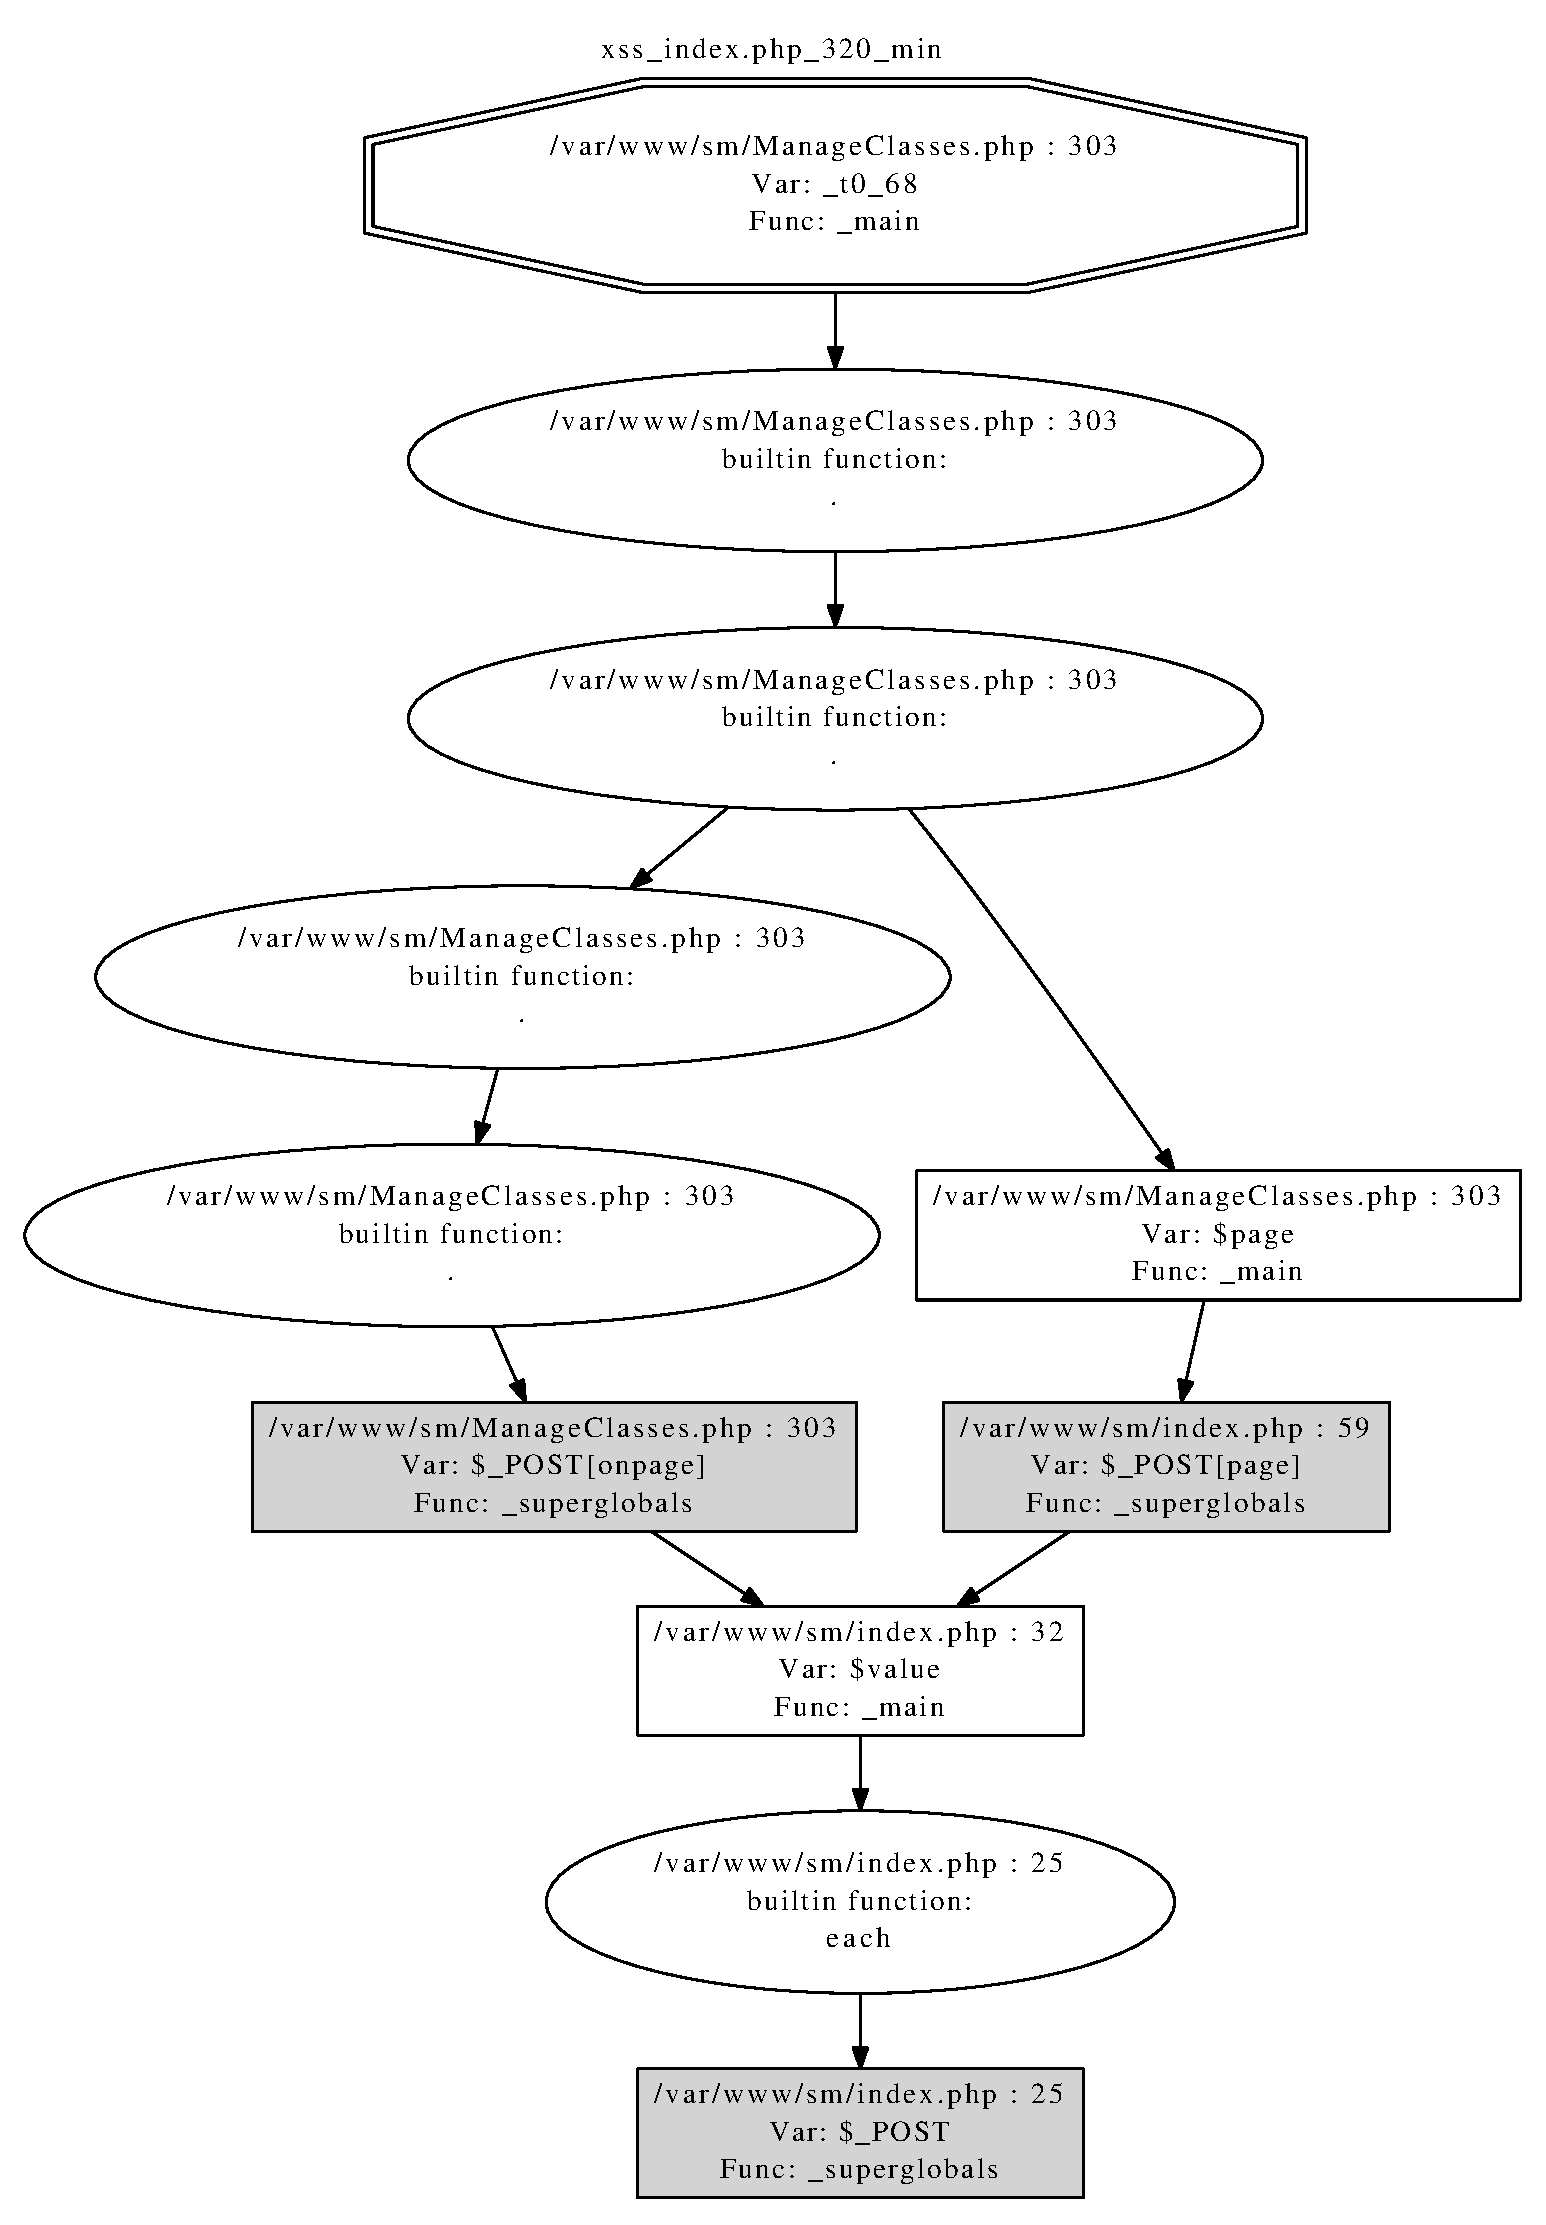
\includegraphics[scale=.3]{320}
	\end{center}
\end{figure}
\\All the POST variables now are inserted into \$value when the \textit{sanitization block} of Listing~\ref{lst:sanblock} is performed. But the \$value variable is just used to sanitize the post and is not used elsewhere, so all of these new cases are false positives.
\end{homeworkProblem}
\end{document}
